\chapter{Machine Learning}

\section{Introduction}
The world of today is generating huge amounts of data
as it goes along,
and more and more of it is put to use.
It's quite probable that any consumer in our society
that goes shopping,
uses some kind of service,
or uses the internet
on a daily basis
performs actions that end up in a database.
Not only do persons generate data,
so does everything else we monitor,
and our society happens to monitor quite a lot.
This data is invaluable for any organization that benefits
from information,
and truly, most do.
It is used by financial institutions like insurance companies,
medical institutions, commercial companies, scientific research
and everything in between.
Evidently, as the need for knowledge (or awareness thereof)
increases, so must our abilities to uncover it,
making machine learning an incredibly interesting topic
in today's world.


People are good at creating hypotheses
about what things mean,
connecting the dots
and predicting cause or outcome.
Yet we can only cope
with so much data at a time
and without direction,
the answers we seek may elude us.
Enter the computing device,
programmable to our needs.
Computer programs often take the form
of our expert knowledge put to detailed writing
but they can also cover the gaps where
we don't have the knowledge
and instead need to uncover it.
This includes anything of valuable information to us,
be it patterns in certain data or hypotheses for predictions.
Where the domain expert describes such hypotheses
using a computer program,
the machine learning expert devises ways of uncovering
the hypotheses.
Evidently, the power of computers would be much greater
if they would be made able to learn as we do.

Great advances have already been made in the domain,
yet we have not managed to make computers learn
as well as humans do,
at least not in as many regards as we do.
The best applications do, however,
get better results than humans in very specific domains.


\paragraph{}
Machine learning is a collection of methods
used to bridge the aforementioned gap
between data and knowledge.
A machine learning algorithm learns from data
and learns an hypothesis or model on it,
which can then be used to make predictions on future data.
This separates it from other algorithms
designed by an expert
that follow a static rule set.
It is inherently an interdisciplinary field,
with its roots firmly embedded
in a statistical foundation
combined with AI,
drawing inspiration from fields such as
information theory,
complexity theory,
psychology
and other fields.

The rest of this chapter will describe the basics of machine learning
along with the specific tools I will use throughout this thesis.
The foundation should be quite sufficient to build up
an understanding of the field
so as to allow the reader to follow the following chapters comfortably.
Next to exploring a foundation,
I will describe specific methods such as neural networks
and convolutional layers,
both exciting techniques that will be used further on.
However, perhaps to the reader's delight,
a cursory glance at the high-level introduction of these methods
should suffice for the reader who only seeks to understand
the applications described herein.
The careful reader is of course cordially invited
to read the more detailed descriptions.


\section{Hands-on Introduction}
A machine learning algorithm
is usually required to form hypotheses
based on given observations.
In this way it can be seen as
a black-box oracle
in which data are shoved
and answers pop out.
Let's take as an easy example
the probably overused and dead-beaten weather forecast.

Let's say we only need to do a daily forecast.
Data come in in the form of meteorological observations
such as temperature, wind speed, and whatever else
experts observe to make top-notch predictions.
This then gets paired
with a description of the actual weather the next day.
Together they form experience-target pairs
$(x_i, y_i)$
that correspond to a meteorological observation
on the one day and the weather on the next day,
in the hope that we can somehow deduct the hidden
link between the two.
The target $y_i$ is what we're really after
so we should choose carefully as to what we are trying to predict.
$y_i$ can be a nominal value,
i.e. from a given set of values
such as the set $(sunny, rainy, windy)$,
in which case the problem is called a \textit{classification} problem.
Contrarily, it can be a real-valued number such as temperature
in which case we call the problem a \textit{regression} problem.
The distinction is worth nothing because
some techniques lend themselves well to
one category but not necessarily to the other.
On this data we will try to learn a hypothesis $h$
that can predict the target weather $y$
for any given observation $x$.
Now all we need to do is fill in the bits in between.

We already have a vague description of what we want to achieve
but now we need to design the problem.
Let us pick for our targets the real-valued temperature some day.
The observations, or \textit{features}, we will base our model on
will take the form of a vector
$(Temperature, Sky, Wind)$ or $(x_1, x_2, x_3)$ short,
where $Temperature$ and $Wind$ are real-valued,
whereas $Sky$ takes on one of the three values
$(Sunny, Rainy, Cloudy)$.
Now we need some kind of function connecting
observation to target.
One of the easiest choices would be a linear
function that combines the features
and outputs the target we are looking for.
It would look quite simple:

$$ y = w_0 + w_1x_1 + w_2x_2 + w_3x_3 $$

We are still stuck with the problem that $x_2$, or $Sky$,
is a nominal value and therefore does not fit all too well with algebra.
We can work around this by agreeing on
a little preprocessing step
that maps $Sunny$ to $-1$, $Rainy$ to $0$ and $Cloudy$ to $1$.
Now that our model is defined, all that is left for us to do
is train it.

In order to train our model we need a data set with training examples
$(x_i, y_i)$,
where the temperature $y_i$ corresponds to
the observations $x_i$ the previous day.
All that remains now is to pick the best weights
so the resulting model is the best hypothesis.
We describe a \textit{best fit}
we need some metric of performance.
The easiest one available is the error on the predictions made by the model
compared to the targets in the training data.
The best hypothesis is the one that minimizes this error.
The most common error by far is the \textit{mean squared error},
though others certainly exist.
Given a training set $D$, it is defined as follows:

$$ E = \frac{1}{|D|} \sum_{(x_i, y_i) \in D}{(h(x_i) - y_i)^2} $$

Multiple algorithms exist that minimize $E$ in such a manner.
If all data is available in one go, as it is in our case,
we can simply apply linear regression to our system
of $|D|$ equations $y = xw$ in order to find a $w$
with the lowest error.
Why not just go for an error of $0$?
We could, however it is unlikely since we suffer from two problems:
insufficient data and a delusion of a perfect world.
In other words, our features probably are not sufficient
and our data is noisy.
If we still manage a training error of $0$
we probably committed the grave mistake of
\textit{overfitting} the training data,
meaning we included the noise of the data in our model.
The reason this is to be avoided is that noise
cannot be predicted by definition and a model that tries
to do so will perform even worse on similar unseen samples.

< TODO image of overfitting >

An alternative algorithm to find our optimal weights $w$
is the \textit{weight update rule},
a source of inspiration for many more algorithms.
The idea behind is that every sample
you calculate your prediction
and shift the weights in the direction of the error,
proportionally to the size of the error.
So, for every sample:
\begin{enumerate}
\item Calculate $\hat{y_i} = h(x_i)$
\item Update $w_i = w_i + \eta(y_i - \hat{y_i})x_i$
\end{enumerate}

The update size can be tweaked with $\eta$.

\paragraph{}
As you have witnessed yourself,
designing a machine learning task
is rather an art than an exact science.
The first optimization algorithm proposed,
linear regression,
is only available for linear models.
Finding the ultimate weights
makes more sense in a regression context
as opposed to a classification context.

There are many more such decisions to made
and models to choose from.
During the next sections,
I will touch on some interesting
models that are used throughout this thesis.

\section{Bias and Variance}
%TODO

\section{Curse of Dimensionality}
The distance between two instances is calculated based on all their attributes.
For these instances to have a small distance between them,
they should be close to one another in all of their attributes,
or otherwise put,
they should be similar in all aspects.
The more attributes or dimensions they have,
the harder this becomes.
This informally introduced phenomenon we call
the \textit{curse of dimensionality}.



\section{Artificial Neural Networks}
Neural networks provide a robust method to learn
vector-valued target functions.
% TODO more examples is better
They have effectively been used for a multitude of machine learning domains,
including recognition of handwritten characters
\cite{LeCun1989}
and
face recognition
\cite{Cottreil1991},
but also in reinforcement learning
(\cite{anderson1989}, \cite{lin1993}). % inverted pendulum
Both popularity and effectiveness of neural networks can be attributed to
their ability to cope with noisy, real-world data,
as well as being able to approximate any function,
albeit with possibly very large complexity (TODO ref).
% TODO maybe pic
\paragraph{}
In part, they are man's attempt
to model the biology of the brain,
or at least that is where the inspiration came from.
The artificial neural networks we construct
consist of interconnected units,
each taking in real-valued inputs
and outputting a real value,
possibly connecting to multiple other units.
This can be in a directed, feed-forward manner,
but it does not have to be.
Interesting architectures have been discovered
that make use of recurrent connections.
Such architectures will be considered in (TODO link).
To complete the analogy,
the human brain consists of a large amount of densely packed neurons,
approximately $10^{11}$ in total.
Compared to an artificial neuron,
they fire a lot slower
yet still humans are capable of
making incredibly complicated decisions
(or recognitions)
in a matter of less than a second.
This hints at great parallelism,
an attribute that is still important
in the artificial neural networks we construct,
especially in real-life situation reinforcement learning
where decisions must be made swiftly and we cannot wait
for a slower model to finish computing.
While our general purpose machines 
are entirely sequential in nature,
parallel hardware has been built specially
for neural network applications.
These are not generally available,
as each domain and even each problem
still require their own specific architectures.
Still, in modern day, many make use
of the parallel capabilities of
Graphic Processing Units (GPUs),
effectively making artificial neural networks even more useful.

The analogy is limited however.
Our use of neural networks draws inspiration from nature
but does not aim to mimic perfectly.
Whereas our neural networks output real values,
biological neurons produce a series of spikes
where both timing and intensity impact the result, % TODO citatie :/?
a phenomenon researchers are still trying to model perfectly.
For now,
we shall content ourselves without the dimension of time.

\subsection{Perceptron}
Artificial neural networks are made up of simple elements called units.
Units are connected through directed connections
that are associated with a weight.
These weights are what make up the parameters of the model.
Units are usually divided in layers depending on their function
and location within the network.
Non-input units get their activation signal, i.e. their input,
from some function of the values of the incoming connections
and the weights associated with them.

\begin{figure}
\label{fig.neuralnet}
\center
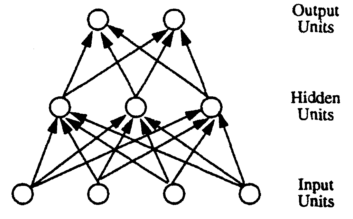
\includegraphics[]{net.png}
\caption{Multi-layer neural network with a single hidden layer.}
\end{figure}

%TODO ref on perceptrons
Activation functions can be linear or nonlinear.
A special kind of unit is the \textit{perceptron},
which outputs either a $-1$ or $1$,
depending on the value of a linear combination of the input:

\begin{equation}
\label{eq.perceptron}
o(\overrightarrow{x}) = \begin{cases}
1 & if \overrightarrow{w}\cdot\overrightarrow{x} > 0 \\
-1 & otherwise
\end{cases}
\end{equation}

\begin{figure}
\label{fig.ml.perceptron}
\center
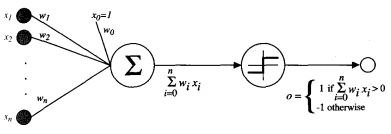
\includegraphics[]{perceptron.png}
\caption{Basic perceptron unit.}
%TODO accredit
\end{figure}

%TODO I have the perceptron img, need to clean and attribute properly
where $\overrightarrow{w}$ denotes the weights of the incoming connection
and $\overrightarrow{x}$ the corresponding incoming values.
This function effectively creates a hyperplane decision surface;
it separates the input space in two.

\subsection{Sigmoid}
A problem with perceptrons
is that they are not differentiable
in their whole domain.
As I'll explain further down, %TODO ref
differentiability is a useful and ofttimes required attribute.
As a way to circumvent this difficulty of non-differentiability,
the \textit{sigmoid} (denoted $\sigma(x)$) is often used:

\begin{equation}
\label{eq.ml.sigmoid}
\sigma(x) = \frac{1}{1 + e^{-x}}
\end{equation}

\begin{figure}[h]
\center
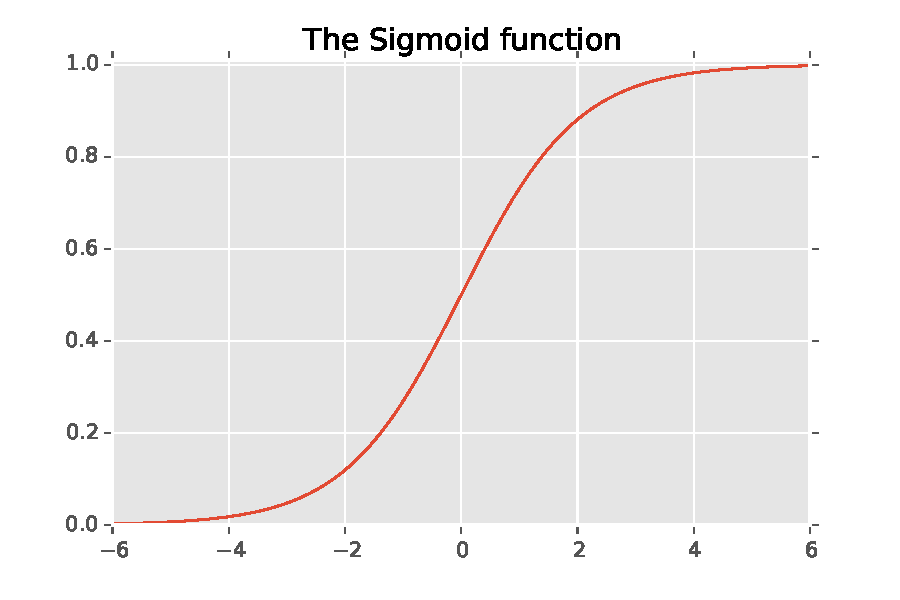
\includegraphics[width=.7\textwidth]{sigmoid.pdf}
\caption{The Sigmoid function}
\label{fig.ml.sigmoid}
\end{figure}

%TODO img of sigmoid
As can be seen on fig \ref{fig.ml.sigmoid},
it has the same tendency as the perceptron activation function
to separate the input space in two
but there is a transition area of uncertainty between the two extremes,
allowing the function to be differentiable in its whole domain.

\subsection{Hyperbolic Tangent}

\subsection{Rectified Linear Unit}

\subsection{Gradient Descent and Backpropagation}

\subsection{Convolutional Neural Networks}

\subsection{Recurrent Neural Networks}

\section{•}